\documentclass{standalone}
\usepackage{tikz}
\usetikzlibrary{patterns, positioning}


\begin{document}
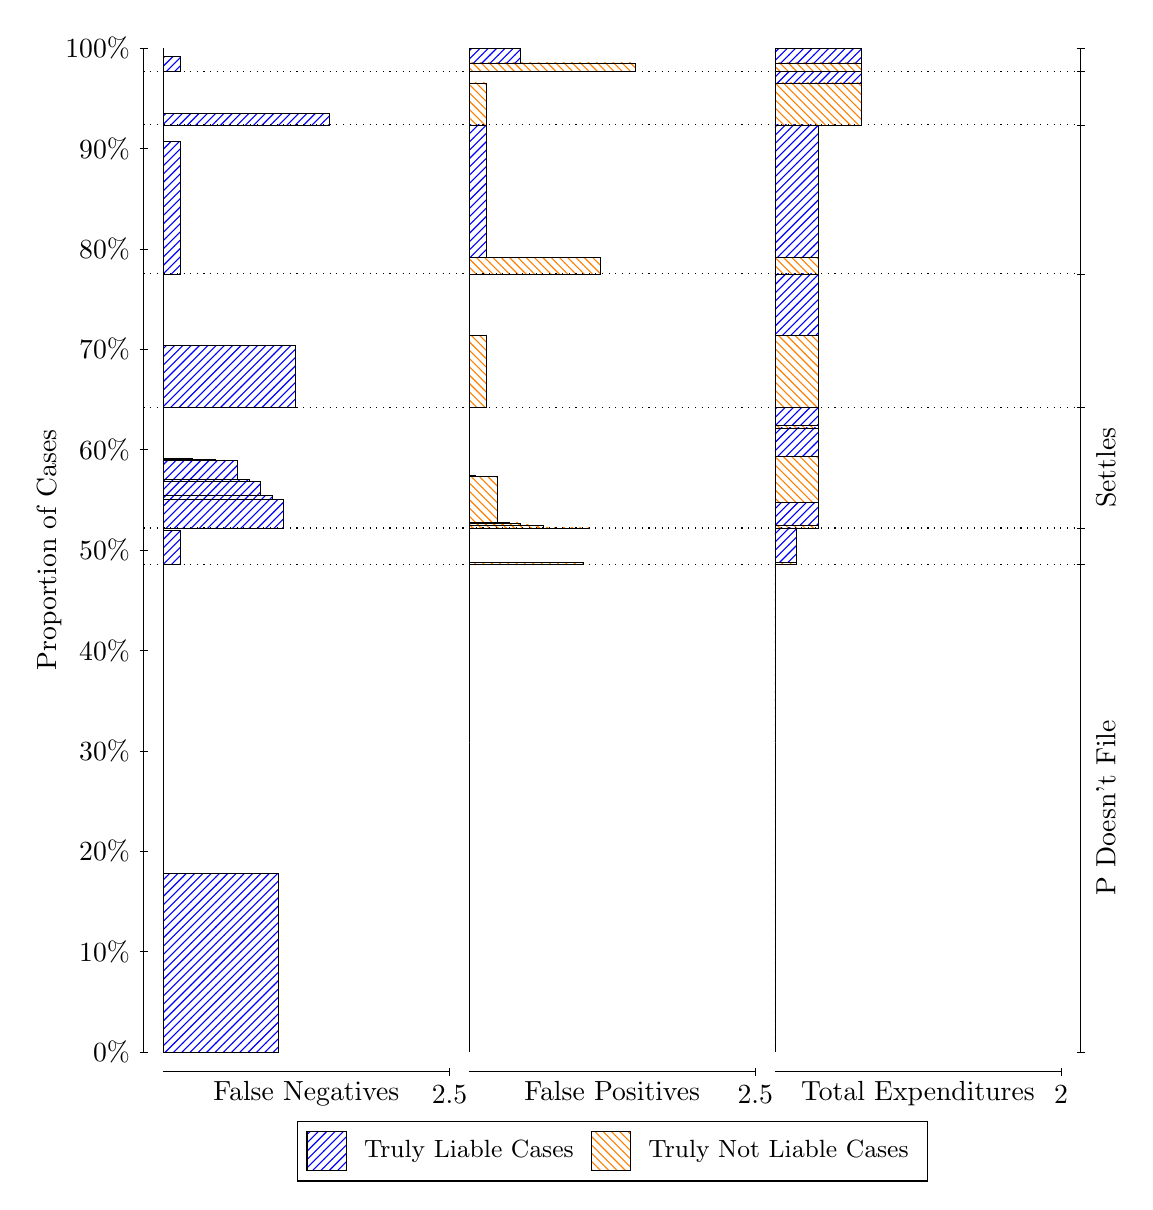
\begin{tikzpicture}
\draw[black, very thin] (1.5,1.75) -- (1.5,14.5);
\node[rotate=90, text=black, anchor=center] at (0.3, 8.125) {Proportion of Cases};
\draw[black, very thin] (1.45,1.75) -- (1.55,1.75);
\node[text=black, anchor=east] at (1.45, 1.75) {0\%};
\draw[black, very thin] (1.45,3.025) -- (1.55,3.025);
\node[text=black, anchor=east] at (1.45, 3.025) {10\%};
\draw[black, very thin] (1.45,4.3) -- (1.55,4.3);
\node[text=black, anchor=east] at (1.45, 4.3) {20\%};
\draw[black, very thin] (1.45,5.575) -- (1.55,5.575);
\node[text=black, anchor=east] at (1.45, 5.575) {30\%};
\draw[black, very thin] (1.45,6.85) -- (1.55,6.85);
\node[text=black, anchor=east] at (1.45, 6.85) {40\%};
\draw[black, very thin] (1.45,8.125) -- (1.55,8.125);
\node[text=black, anchor=east] at (1.45, 8.125) {50\%};
\draw[black, very thin] (1.45,9.4) -- (1.55,9.4);
\node[text=black, anchor=east] at (1.45, 9.4) {60\%};
\draw[black, very thin] (1.45,10.675) -- (1.55,10.675);
\node[text=black, anchor=east] at (1.45, 10.675) {70\%};
\draw[black, very thin] (1.45,11.95) -- (1.55,11.95);
\node[text=black, anchor=east] at (1.45, 11.95) {80\%};
\draw[black, very thin] (1.45,13.225) -- (1.55,13.225);
\node[text=black, anchor=east] at (1.45, 13.225) {90\%};
\draw[black, very thin] (1.45,14.5) -- (1.55,14.5);
\node[text=black, anchor=east] at (1.45, 14.5) {100\%};

\draw[black, very thin] (13.4,1.75) -- (13.4,14.5);
\draw[black, very thin] (13.35,1.75) -- (13.45,1.75);
\node[anchor=west] at (13.35, 1.75) {};
\draw[black, very thin] (13.35,7.9452) -- (13.45,7.9452);
\node[anchor=west] at (13.35, 7.9452) {};
\draw[black, very thin] (13.35,8.4046) -- (13.45,8.4046);
\node[anchor=west] at (13.35, 8.4046) {};
\draw[black, very thin] (13.35,9.9379) -- (13.45,9.9379);
\node[anchor=west] at (13.35, 9.9379) {};
\draw[black, very thin] (13.35,11.633) -- (13.45,11.633);
\node[anchor=west] at (13.35, 11.633) {};
\draw[black, very thin] (13.35,13.524) -- (13.45,13.524);
\node[anchor=west] at (13.35, 13.524) {};
\draw[black, very thin] (13.35,14.201) -- (13.45,14.201);
\node[anchor=west] at (13.35, 14.201) {};
\draw[black, very thin] (13.35,14.5) -- (13.45,14.5);
\node[anchor=west] at (13.35, 14.5) {};

\draw[black, very thin, pattern color=blue, pattern=north east lines] (1.75,1.75) rectangle (3.2033,4.0147);
\draw[black, very thin, pattern color=orange, pattern=north west lines] (1.75,4.0147) rectangle (1.75,7.9452);
\draw[black, very thin, pattern color=blue, pattern=north east lines] (1.75,7.9452) rectangle (1.968,8.3788);
\draw[black, very thin, pattern color=orange, pattern=north west lines] (1.75,8.3788) rectangle (1.75,8.4046);
\draw[black, very thin, pattern color=blue, pattern=north east lines] (1.75,8.4046) rectangle (3.276,8.7679);
\draw[black, very thin, pattern color=blue, pattern=north east lines] (1.75,8.7679) rectangle (3.1307,8.8166);
\draw[black, very thin, pattern color=blue, pattern=north east lines] (1.75,8.8166) rectangle (2.9853,8.9954);
\draw[black, very thin, pattern color=blue, pattern=north east lines] (1.75,8.9954) rectangle (2.84,9.0242);
\draw[black, very thin, pattern color=blue, pattern=north east lines] (1.75,9.0242) rectangle (2.6947,9.2648);
\draw[black, very thin, pattern color=blue, pattern=north east lines] (1.75,9.2648) rectangle (2.5493,9.2667);
\draw[black, very thin, pattern color=blue, pattern=north east lines] (1.75,9.2667) rectangle (2.404,9.2712);
\draw[black, very thin, pattern color=blue, pattern=north east lines] (1.75,9.2712) rectangle (2.2587,9.2731);
\draw[black, very thin, pattern color=blue, pattern=north east lines] (1.75,9.2731) rectangle (2.1133,9.284);
\draw[black, very thin, pattern color=orange, pattern=north west lines] (1.75,9.284) rectangle (1.75,9.9379);
\draw[black, very thin, pattern color=blue, pattern=north east lines] (1.75,9.9379) rectangle (3.4213,10.72);
\draw[black, very thin, pattern color=orange, pattern=north west lines] (1.75,10.72) rectangle (1.75,11.633);
\draw[black, very thin, pattern color=blue, pattern=north east lines] (1.75,11.633) rectangle (1.968,13.314);
\draw[black, very thin, pattern color=orange, pattern=north west lines] (1.75,13.314) rectangle (1.75,13.524);
\draw[black, very thin, pattern color=blue, pattern=north east lines] (1.75,13.524) rectangle (3.8573,13.67);
\draw[black, very thin, pattern color=orange, pattern=north west lines] (1.75,13.67) rectangle (1.75,14.201);
\draw[black, very thin, pattern color=blue, pattern=north east lines] (1.75,14.201) rectangle (1.968,14.39);
\draw[black, very thin, pattern color=orange, pattern=north west lines] (1.75,14.39) rectangle (1.75,14.5);
\draw[black, very thin, pattern color=orange, pattern=north west lines] (5.6333,1.75) rectangle (5.6333,5.6805);
\draw[black, very thin, pattern color=blue, pattern=north east lines] (5.6333,5.6805) rectangle (5.6333,7.9452);
\draw[black, very thin, pattern color=orange, pattern=north west lines] (5.6333,7.9452) rectangle (7.0867,7.971);
\draw[black, very thin, pattern color=blue, pattern=north east lines] (5.6333,7.971) rectangle (5.6333,8.4046);
\draw[black, very thin, pattern color=orange, pattern=north west lines] (5.6333,8.4046) rectangle (7.1593,8.4052);
\draw[black, very thin, pattern color=orange, pattern=north west lines] (5.6333,8.4052) rectangle (7.014,8.4053);
\draw[black, very thin, pattern color=orange, pattern=north west lines] (5.6333,8.4053) rectangle (6.8687,8.4056);
\draw[black, very thin, pattern color=orange, pattern=north west lines] (5.6333,8.4056) rectangle (6.7233,8.4057);
\draw[black, very thin, pattern color=orange, pattern=north west lines] (5.6333,8.4057) rectangle (6.578,8.4387);
\draw[black, very thin, pattern color=orange, pattern=north west lines] (5.6333,8.4387) rectangle (6.4327,8.4428);
\draw[black, very thin, pattern color=orange, pattern=north west lines] (5.6333,8.4428) rectangle (6.4327,8.4428);
\draw[black, very thin, pattern color=orange, pattern=north west lines] (5.6333,8.4428) rectangle (6.2873,8.4706);
\draw[black, very thin, pattern color=orange, pattern=north west lines] (5.6333,8.4706) rectangle (6.142,8.4768);
\draw[black, very thin, pattern color=orange, pattern=north west lines] (5.6333,8.4768) rectangle (5.9967,9.0586);
\draw[black, very thin, pattern color=blue, pattern=north east lines] (5.6333,9.0586) rectangle (5.706,9.0694);
\draw[black, very thin, pattern color=blue, pattern=north east lines] (5.6333,9.0694) rectangle (5.6333,9.9379);
\draw[black, very thin, pattern color=orange, pattern=north west lines] (5.6333,9.9379) rectangle (5.8513,10.851);
\draw[black, very thin, pattern color=blue, pattern=north east lines] (5.6333,10.851) rectangle (5.6333,11.633);
\draw[black, very thin, pattern color=orange, pattern=north west lines] (5.6333,11.633) rectangle (7.3047,11.844);
\draw[black, very thin, pattern color=blue, pattern=north east lines] (5.6333,11.844) rectangle (5.8513,13.524);
\draw[black, very thin, pattern color=orange, pattern=north west lines] (5.6333,13.524) rectangle (5.8513,14.056);
\draw[black, very thin, pattern color=blue, pattern=north east lines] (5.6333,14.056) rectangle (5.6333,14.201);
\draw[black, very thin, pattern color=orange, pattern=north west lines] (5.6333,14.201) rectangle (7.7407,14.311);
\draw[black, very thin, pattern color=blue, pattern=north east lines] (5.6333,14.311) rectangle (6.2873,14.5);
\draw[black, very thin, pattern color=orange, pattern=north west lines] (9.5167,1.75) rectangle (9.5167,5.6805);
\draw[black, very thin, pattern color=blue, pattern=north east lines] (9.5167,5.6805) rectangle (9.5167,7.9452);
\draw[black, very thin, pattern color=orange, pattern=north west lines] (9.5167,7.9452) rectangle (9.7892,7.971);
\draw[black, very thin, pattern color=blue, pattern=north east lines] (9.5167,7.971) rectangle (9.7892,8.4046);
\draw[black, very thin, pattern color=orange, pattern=north west lines] (9.5167,8.4046) rectangle (10.062,8.4428);
\draw[black, very thin, pattern color=blue, pattern=north east lines] (9.5167,8.4428) rectangle (10.062,8.7303);
\draw[black, very thin, pattern color=orange, pattern=north west lines] (9.5167,8.7303) rectangle (10.062,9.3121);
\draw[black, very thin, pattern color=blue, pattern=north east lines] (9.5167,9.3121) rectangle (10.062,9.6754);
\draw[black, very thin, pattern color=orange, pattern=north west lines] (9.5167,9.6754) rectangle (10.062,9.7094);
\draw[black, very thin, pattern color=blue, pattern=north east lines] (9.5167,9.7094) rectangle (10.062,9.9379);
\draw[black, very thin, pattern color=orange, pattern=north west lines] (9.5167,9.9379) rectangle (10.062,10.851);
\draw[black, very thin, pattern color=blue, pattern=north east lines] (9.5167,10.851) rectangle (10.062,11.633);
\draw[black, very thin, pattern color=orange, pattern=north west lines] (9.5167,11.633) rectangle (10.062,11.844);
\draw[black, very thin, pattern color=blue, pattern=north east lines] (9.5167,11.844) rectangle (10.062,13.524);
\draw[black, very thin, pattern color=orange, pattern=north west lines] (9.5167,13.524) rectangle (10.607,14.056);
\draw[black, very thin, pattern color=blue, pattern=north east lines] (9.5167,14.056) rectangle (10.607,14.201);
\draw[black, very thin, pattern color=orange, pattern=north west lines] (9.5167,14.201) rectangle (10.607,14.311);
\draw[black, very thin, pattern color=blue, pattern=north east lines] (9.5167,14.311) rectangle (10.607,14.5);
\draw[black, dotted] (1.5,7.9452) -- (13.4,7.9452);
\draw[black, dotted] (1.5,8.4046) -- (13.4,8.4046);
\draw[black, dotted] (1.5,9.9379) -- (13.4,9.9379);
\draw[black, dotted] (1.5,11.633) -- (13.4,11.633);
\draw[black, dotted] (1.5,13.524) -- (13.4,13.524);
\draw[black, dotted] (1.5,14.201) -- (13.4,14.201);
\draw[black, very thin] (1.75,1.5) -- (5.3833,1.5);
\node[text=black, anchor=north] at (3.5667, 1.5) {False Negatives};
\draw[black, very thin] (5.3833,1.45) -- (5.3833,1.55);
\node[text=black, anchor=north] at (5.3833, 1.45) {2.5};

\draw[black, very thin] (5.6333,1.5) -- (9.2667,1.5);
\node[text=black, anchor=north] at (7.45, 1.5) {False Positives};
\draw[black, very thin] (9.2667,1.45) -- (9.2667,1.55);
\node[text=black, anchor=north] at (9.2667, 1.45) {2.5};

\draw[black, very thin] (9.5167,1.5) -- (13.15,1.5);
\node[text=black, anchor=north] at (11.333, 1.5) {Total Expenditures};
\draw[black, very thin] (13.15,1.45) -- (13.15,1.55);
\node[text=black, anchor=north] at (13.15, 1.45) {2};

\node[text=black, centered, rotate=90] at (13.72, 4.8476) {P Doesn't File};

\node[text=black, centered, rotate=90] at (13.72, 9.1713) {Settles};





\draw (7.449999999999999,1.5) node[draw=none] (baseCoordinate) {};
\begin{scope}[align=center]
        \matrix[scale=0.5, draw=black, below=0.5cm of baseCoordinate, nodes={draw}, column sep=0.1cm]{
            \node[rectangle, draw, minimum width=0.5cm, minimum height=0.5cm, pattern color=blue, pattern=north east lines] {}; &
            \node[draw=none, font=\small, text=black] (B) {Truly Liable Cases}; &
            \node[rectangle, draw, minimum width=0.5cm, minimum height=0.5cm, pattern color=orange, pattern=north west lines] {}; &
            \node[draw=none, font=\small, text=black] (B) {Truly Not Liable Cases}; \\
            };
\end{scope}

\end{tikzpicture}
\end{document}